\section{Method}
\label{sec:method}
The fundamental algorithm of DLA, as described by Witten \& Sanders \cite{PhysRevLett.47.1400} is as follows; a seed particle (the particle we follow) is placed at the centre. This particle will be the basis of the growing cluster. Another particle is then introduced at some distance from this seeding particle. The starting position of this particle can in principle be infinitely far away from the particle, but for practical matters, it is often placed close to the seeding particle. This particle will perform a random walk in the space around the seeding particle, with the intention that at some point in time, the walking particle will hit (i.e. be sufficiently close to) the seeding particle, and the two will clump together. 

All of the following algorithms have been implemented using C++ 14. \textcolor{red}{??? Don't know about the following part, but:} The code was run on OS X Yosemite 2,7 GHz Intel Core i5 8 GB 1867 MHz DDR3 system.

\subsection{On-lattice DLA}
\label{sec:on-lattice_method}
For the on-lattice case, the algortihm is pretty straight forward, as is described in the beginning of section \ref{sec:method}. Thus it will only briefly be discussed here, with the main focus being on the off-lattice version. Special for the on-lattice case is that the particle can only move in discrete steps and directions. That is, it may only move along the axis (either north, south, east or west), but not diagonally. More specific for the simulation run in this project is that the walking particles would always start at a random (uniformly distributed) point on the perimeter of the grid. If it was to take a step causing it to move outside of the grid, it would restart somewhere else on the perimeter. Although this cannot be done without some loss of generality, it is still done to increase the simulation speed. \textcolor{red}{??? should look into this more?}

Since the on-lattice simulation is of less interest compared to the off-lattice case, only a crude on-lattice simulation was performed. The results of the on-lattice simulations can be found in \textcolor{red}{??? Link to section with results for on-lattice DLA simulations. }

\subsection{Off-lattice DLA}
In off-lattice DLA simulations, the particle is no longer restricted to move along any axis. This means it can move freely in an approximately continous space, and any direction. This makes the algorithm is more advanced than the on-lattice one. The algorithm used for the off-lattice DLA simulation is based on the one suggested by Kuijpers et. al. \cite{Kuijpers2014841}. In this algorithm, one uses an on-lattice approximation for storing the positions of the particles in the cluster, thus being more RAM dependant than other algorithms, but with the benefit of reducing the calculation of sites viable for hits. Like in section \ref{sec:on-lattice_method}, the particle starts along a circle of radius $R_{start}$ from the cluster, and will be killed if the wander too far from the cluster. This limit is set to $R_{kill} = 5R_{cluster}$, where $R_{cluster}$ is the radius of the smallest circle spanning the cluster.

The concept is as follows: The program uses three arrays (illustrated in figure \ref{fig:arrays}), which together keeps track of all information of interest. The first one, $\textbf{A}$, is an $N \times 2$ array, which only keeps track of the exact coordinates of the particle. These coordinates are then mapped to correspond to integer values, so that they may correspond to a cell number in $\textbf{B}$, an $n \times n$ ($n$ is lattice size) array in which all the elements are either $0$ or the label of the particle. See figure \ref{fig:A_sketch} and \ref{fig:B_array} for an illustration of this. In this context, label refers to the number given to the particle when it attaches to the cluster, starting from the original seed particle. The final array, $\textbf{C}$, stores the distance from each cell to a particle, as shown in figure \ref{fig:C_array}. This is done in order to keep track of the distance from a walking particle to a point on the cluster. The great benefit of this algorithm lies in being able to take steps of varying length, depending on the distance from the cluster, which is only possible without loss of generality if the particle is far away from the cluster. For simplicity, there is a set a maximum distance $D_{max}$ to be the maximum distance cap. This reduces the amount of number of calculations required per iteration. 

\begin{figure}[h]
	\begin{center}
		\begin{subfigure}[t]{0.3\textwidth}
			\includegraphics[width = \textwidth]{fig/A_sketch.png}
			\caption{Illustration of the real situation, where the particles for simplicity allign nicely along the horizontal axis.  }
			\label{fig:A_sketch}
		\end{subfigure}
		\begin{subfigure}[t]{0.3\textwidth}
			\includegraphics[width = \textwidth]{fig/B_array.png}
			\caption{Illustration of how the labelling of the cluster was done. }
			\label{fig:B_array}
		\end{subfigure}
		\begin{subfigure}[t]{0.3\textwidth}
			\includegraphics[width = \textwidth]{fig/C_array.png}
			\caption{Illustration of the rounded off distances at each point in space.  }
			\label{fig:C_array}
		\end{subfigure}
		\caption{Illustration of a dummy configuration of particles, and how each array work. The seed particle is in all cases placed in a $13 \times 13$ array, at position (7,7). For simplicity, the other particles are not random walkers in this dummy case, but move in from right to left, along the horizontal axis.}
		\label{fig:arrays}
	\end{center}
\end{figure}

Throughout the process, the walking particle will take steps depending on its distance from the cluster. The following three criterias determines the different regimes the walker may be in with respect to step size. It is worth noting that $L_{min}$ is the step size taken by the particle corresponding to Brownian motion when the particle is close to the cluster. This value is set before the simulation starts. What regime the particle is in depends on wheter the approximated distance between the walker and the cluster, $d_{wc}$, is so small that there is a chance of hitting the cluster if the particle takes a step of length $L_{min}$. The distance $d_{wc}$ can be found by looking in the cell labeled with the rounded coordinates of the walker in $\textbf{C}$. In addition, one must take into account that what is stored is the coordinates of the centre of the particles, meaning that there must be a distance of $2r_p$ between them at least. Since one looks at the rounded off coordinates in when finding $d_{wc}$, one adds a $1$ to make sure that the region includes all possibilities of hits.

\begin{itemize}
{\setlength\itemindent{1.0in}\item[$d_{wc} \le 2r_p + L_{min} + 1$:] The particle is within hitting range of the cluster. That may be a single particle or lots of particles, and there has to be done an exact calculation for determining if the particle will hit for all of the particles within the range of $d_{wc}$. This is done by looking at all particles stored in $\textbf{B}$ within a square of size $ 2(2r_p + L_{min} + 1)+1$ centered around the cell with indices given by the rounded coordinates of the walking particle. All non-zero elements within this square gives the location of the coordinates in $\textbf{A}$, so they can be extracted. Then the calculation of is the particle hitting is performed for all particles within hitting range, and the one yielding the lowest positive step required will be the one the particle latches on to. 
\item[$ 2r_p + L_{min} + 1 \le  d_{wc} \le D_{max}$:] The particle is in an intermediate position, meaning it can only move a distance of $d_{wc} - (2r_p + L_{min} + 1)$ without having to check for a possibility of a hit. 
\item[$d_{wc} = D_{max}$:] The particle is far away from the cluster, allowing it to move a distance of max($d_{w0} - R_{max} - (2r_p + L_{min} + 1), D_{max} - (2r_p + L_{min} + 1)$).}
\end{itemize}

The particle will attach to the cluster iff the step performed is shorter than $L_{min}$. Then $\textbf{A}$,$\textbf{B}$ and $\textbf{C}$ are updated, and a new particle starts walking. A new walker is launched from the starting distance $R_{start}$, and this process is repeated until the cluster contains the desired amount of particles. 

From the aggregated cluster, the fractal dimension $d_f$ was calculated using a fit of the data to equation \eqref{eq:N_Rg_rel}. 
